\begin{appendices}

\chapter{Material für Nutzerstudie}
\label{appendix:study_material}
\todo{Fragebögen einfügen.}

\begin{figure}[hbt]
    \centering
    \framebox{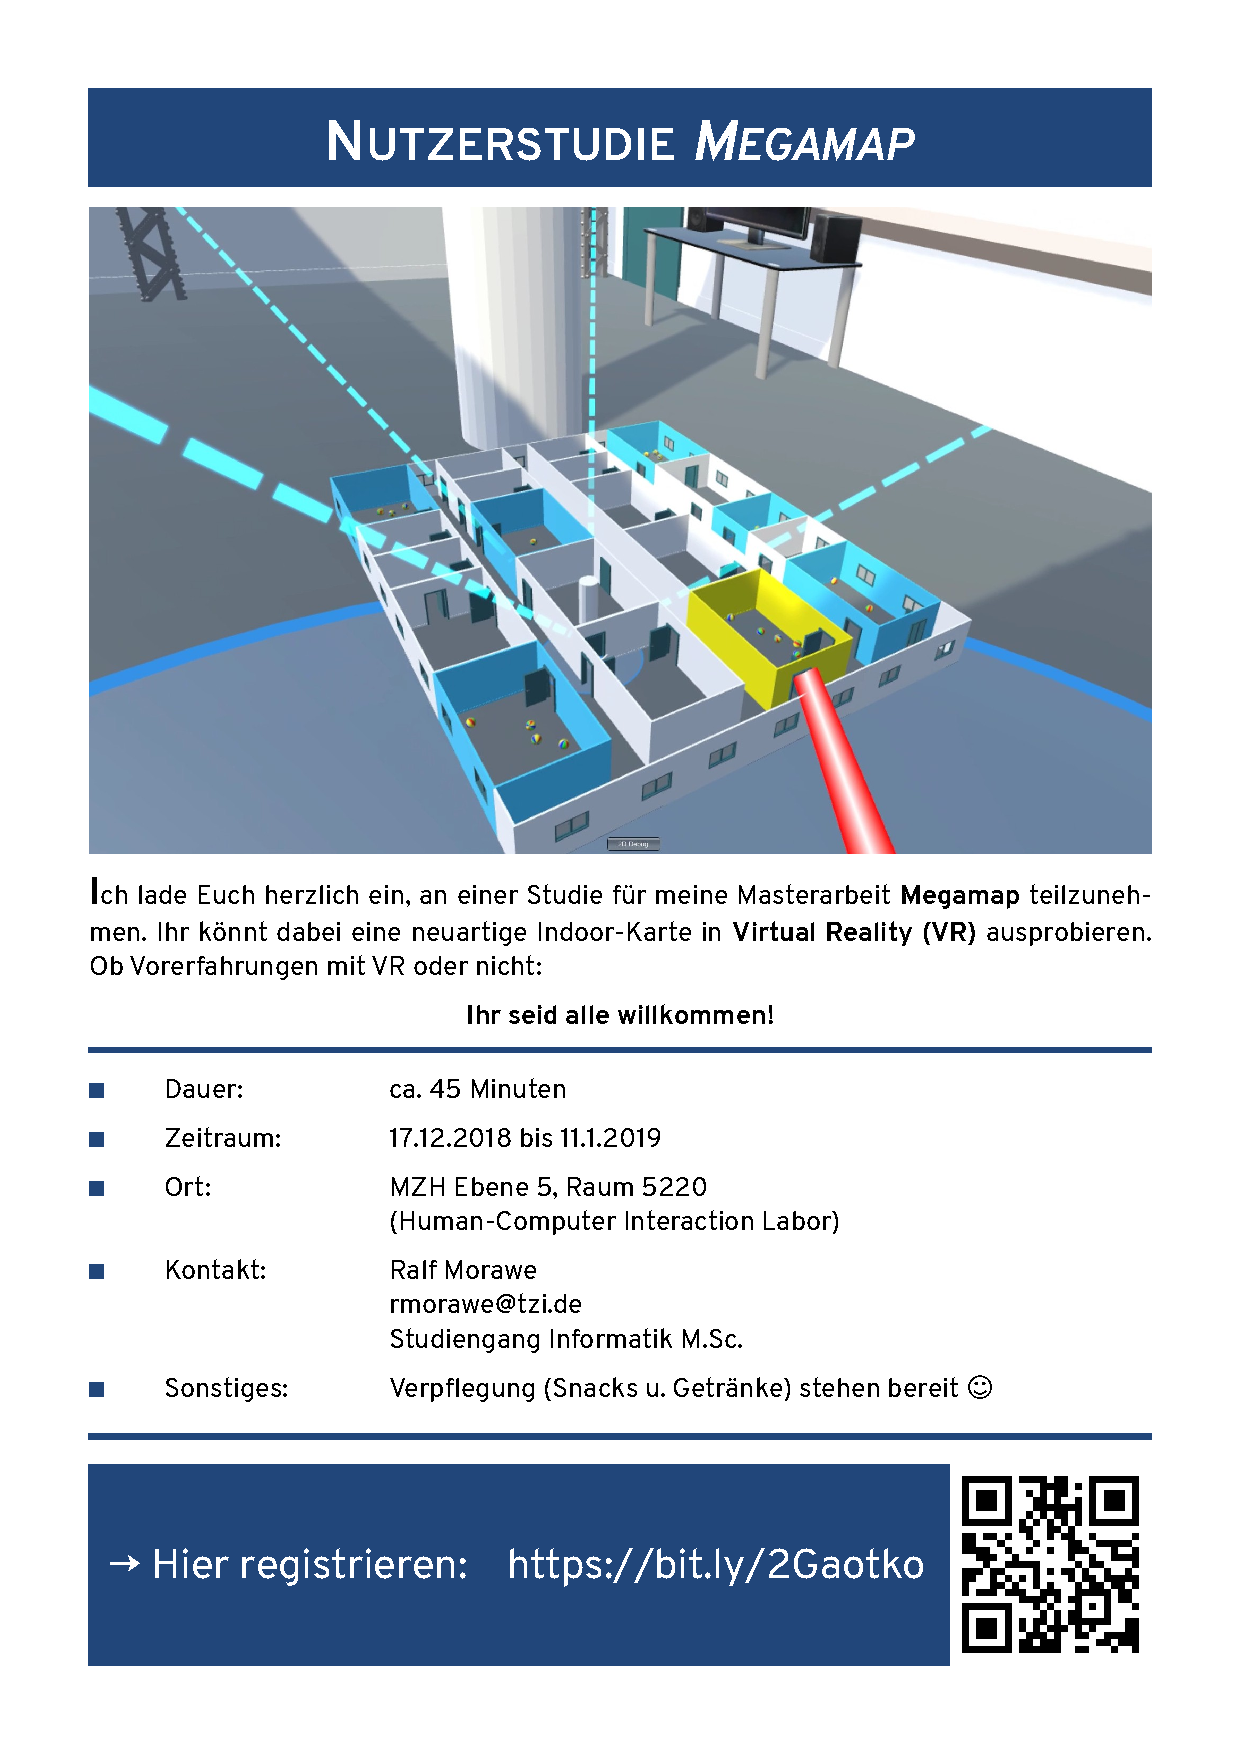
\includegraphics[width=0.725\linewidth]{appendix/study_flyer}}
    \caption{Flyer für Nutzerstudie.}
\end{figure}

\begin{figure}[hbt]
    \centering
    \begin{subfigure}{0.6\linewidth}
        \framebox[\width]{
\includegraphics[page=1, width=\linewidth]{appendix/study_infos}}
    \end{subfigure}

    \begin{subfigure}{0.6\linewidth}
        \framebox[\width]{
\includegraphics[page=2, trim={0, 13cm, 0, 0}, clip, width=\linewidth]{appendix/study_infos}}%
    \end{subfigure}%
    \caption{Informationsbogen für Probanden.}
\end{figure}

\begin{figure}[hbt]
    \centering
    \framebox{
\includegraphics[width=0.725\linewidth]{appendix/Zustimmung-Studienteilnahme}}
    \caption{Zustimmungsbogen für Probanden.}
\end{figure}

\chapter{Konditionssequenzen für die Nutzerstudie}
\begin{table}[h]
    \centering
    \caption{List der Konditionssequenzen für die Probanden.}
    \label{appendix:condition_sequences}
    \begin{tabular}{cccc}\toprule
        Proband & Kondition 1 & Kondition 2 & Kondition 3 \\\midrule
        $P_0$ & $3D_l$ & $3D_h$ & $2D$ \\
        $P_1$ & $3D_h$ & $3D_l$ & $2D$ \\
        $P_2$ & $2D$ & $3D_l$ & $3D_h$ \\
        $P_3$ & $3D_l$ & $2D$ & $3D_h$ \\
        $P_4$ & $3D_h$ & $2D$ & $3D_l$ \\
        $P_5$ & $2D$ & $3D_h$ & $3D_l$ \\
        $P_6$ & $3D_h$ & $2D$ & $3D_l$ \\
        $P_7$ & $3D_l$ & $3D_h$ & $2D$ \\
        $P_8$ & $3D_h$ & $3D_l$ & $2D$ \\
        $P_9$ & $2D$ & $3D_l$ & $3D_h$ \\
        $P_{10}$ & $3D_l$ & $2D$ & $3D_h$ \\
        $P_{11}$ & $2D$ & $3D_h$ & $3D_l$ \\
        $P_{12}$ & $3D_l$ & $3D_h$ & $2D$ \\
        $P_{13}$ & $3D_h$ & $2D$ & $3D_l$ \\
        $P_{14}$ & $2D$ & $3D_l$ & $3D_h$ \\\bottomrule        
    \end{tabular}
\end{table}

\end{appendices}
